\newpage
\section{Object-Oriented Languages} 
面向对象语言 = object-oriented language = OO language = class-based language
\begin{itemize}
    \item (几乎)所有值都是对象(object)
    \item 对象属于某个类, 或者说对象是某个类的实例(instance)
    \item 对象封装了状态(也就是成员变量 fields)与行为(也就是成员方法 methods)
\end{itemize}

重要概念:
\begin{itemize}
    \item 继承(inheritance): 派生类继承基类的特性
    \item 封装(encapsulation): 隐藏不该被外部接触到的接口
    \item 多态(polymorphism): 对象可以以不同形态呈现
\end{itemize}


\subsection{Classes}
拓展 Tiger 以支持对象. 不考大题, 就不详细记了. 


在 Tiger 中实现类需要解决如下问题:
\begin{itemize}
    \item Field layout: 某个类的各个 fields 在内存中如何放置、访问? 换句话说, 如何确定某个实例的 field 内存地址相对这个实例初始地址的偏移量? 
    \item Method dispatch: 调用某个实例的方法时, 如何找到正确的方法位于何地址? 是派生类的实现, 还是基类的实现, 还是基类的基类的实现 ? 
    \item Membership test: 如何检查给定实例是否是给定类的实例? 
\end{itemize}

\subsection{Single Inheritance of Data Fields}
单继承single-inheritance(SI): 每个类最多只能继承一个基类, 因此继承关系图是一棵树. 

\subsubsection{Field layout}
使用 *prefixing

\begin{figure}[!htb]
    \centering
    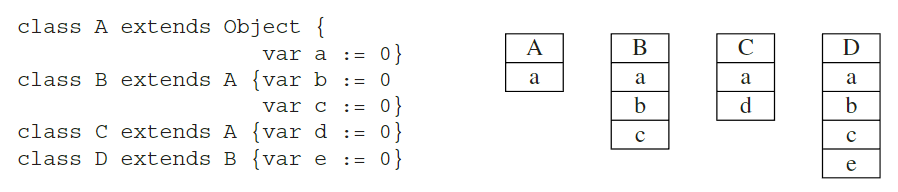
\includegraphics[width=0.42\textwidth]{pic/CP14/Single inheritance of data fields.}
    \caption{Single inheritance of data fields.}
\end{figure}


派生类新增的 fields 跟在基类的后面.  这使得我们可以正确处理多态: 例如把Cat当作Animal看待, 访问Animal的 fields 时相当于屏蔽了新增的 fields; 基类的各个 fields 偏移量不会因为这是个派生类实例发生变化, 仍然是已知的. 这避免了不安全的内存访问. 

\subsubsection{Method dispatch}
每个 method 编译成一段代码(称为 method instance), 编译方式和普通函数几乎无异. 比如 $A$ 中的 $f()$ 就编译为一段代码, 可用 $A_f$ 这样 label 标记函数地址. 机器码中, 函数起始地址使用一个LABEL标出. 

每个类都对应一个 class decriptor, 里面包含了描述这个类的一些必要信息: 
\begin{itemize}
    \item 一个指向基类的指针
    \item 一个列表, 包含这个类所有的 method instances
\end{itemize}

对于 static method 的调用 $x.f()$, 编译器将会: 
\begin{enumerate}
    \item 找到对象 $x$ 对应的类, 记为 $C$.
    \item 如果 $C$ 中有 $f$, 则直接得出 $x.f()$ 翻译结果为 $C_f$; 否则继续向上(在基类中)寻找. 
    \item 假设 $C$ 的基类为 $B$, 在 $B$ 中查找 $f$, 如找到则得出 $x.f()$ 翻译结果为 $B_f$; 否则继续向上(在基类中)寻找. 
    \item $\dots$
    \item 直到在某个祖先中找到为止(或是一路找到Object还没有则报错), 调用它. 
\end{enumerate}

对于 dynamic method 的处理略复杂:
\begin{itemize}
    \item 每个类维护一个 dispatch vector (例如 C++ 中的虚表 vtable = virtual table = VMT = virtual methods table) 储存每个 method 的地址. 
    \subitem 建立方式类似 prefixing: 派生类中新声明的方法跟在基类 dispatch vector 的后面; 不过如果有基类的 method 被重写了, 也要替换成自己重写后 method 的地址. 这样, 每个方法的偏移量是确定的. 
    \item 每个对象都关联某个 vtable: 对象的开头储存一个指针指向对应 class descriptor , 里面就有 vtable. 
    \item 需要动态查找(lookup), 有额外的开销. 
\end{itemize}

\begin{figure}[!htb]
    \centering
    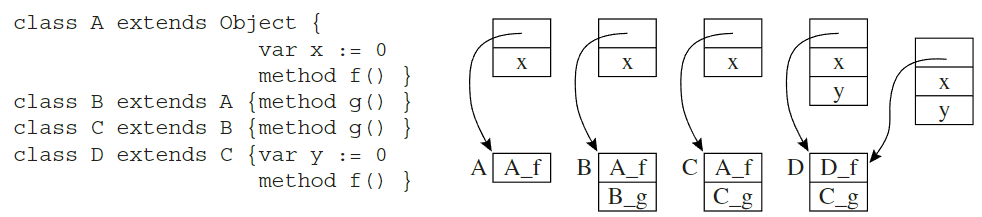
\includegraphics[width=0.42\textwidth]{pic/CP14/Class descriptors for dynamic method lookup}
    \caption{Class descriptors for dynamic method lookup}
\end{figure}

对于 dynamic method 的调用 $x.f()$, 编译器将会: 
\begin{enumerate}
    \item 在 $x$ 的 0 偏移处(开头)找到 class descriptor $d$.
    \item 由于方法 $f$ 的偏移量是确定的(记为 $F$), 从 $d$ 中 $F$ 偏移处获取 $f$ 的函数地址. 
    \item 调用f.
\end{enumerate}

\begin{figure}[!htb]
    \centering
    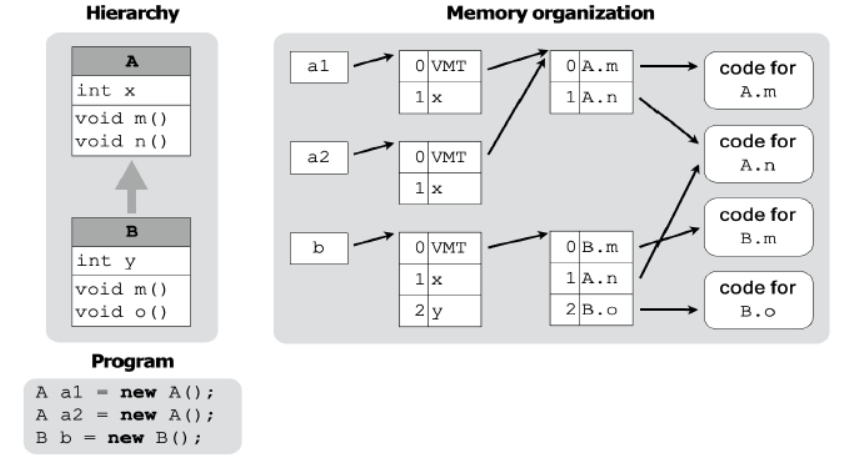
\includegraphics[width=0.309\textwidth]{pic/CP14/dynamic method}
    \caption{dynamic method}
\end{figure}


\subsection{Multiple Inheritance of Data Fields}
多继承multiple-inheritance(MI): 每个类可以继承多个基类, 因此继承关系图是有向无环图(DAG). % 我抄的佬认为多继承是纯纯的方向错误, C++为了多继承打了一堆补丁最后还是破破烂烂. 

\begin{figure}[!htb]
    \centering
    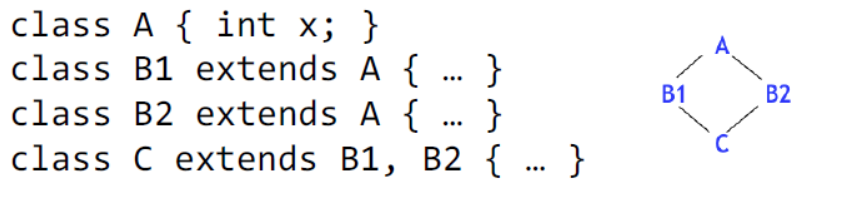
\includegraphics[width=0.309\textwidth]{pic/CP14/菱形继承}
    \caption{菱形继承}
\end{figure}


引入了经典的菱形继承问题: 
\begin{itemize}
    \item 歧义: 如果 $B1$ 和 $B2$ 中都有 method $m$, 那么 $C$ 的实例 $c$ 上调用 $c.m()$ 时应该调用哪个 $m$? 无法确定. 
    \item field replication: 对于 $A$ 中的一个 field $x$, 由于 $B1$ 和 $B2$ 中都继承了 $A.x$, 最终 $C$ 中会有重复的两个 $x$ 都来自 $A$.
\end{itemize}

\subsubsection{Field layout}
通过图染色获取. 

\begin{figure}[!htb]
    \centering
    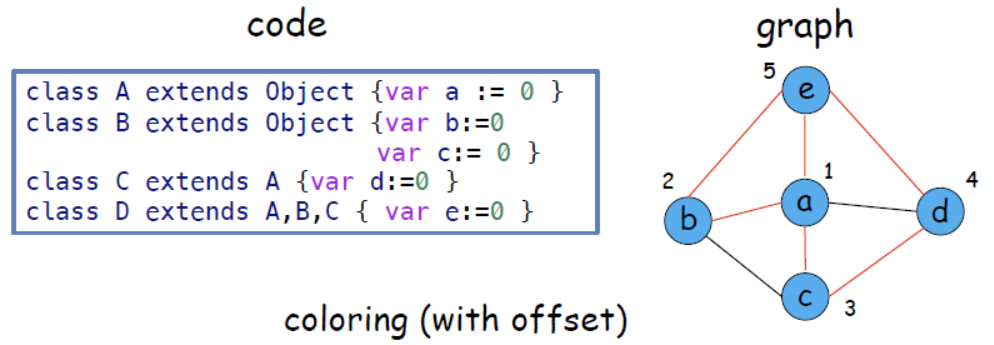
\includegraphics[width=0.42\textwidth]{pic/CP14/Multiple inheritance}
    \caption{Multiple inheritance}
    \label{fig:Multiple inheritance}
\end{figure}

目标: 静态分析所有类, 为每个 field 的找到一个固定偏移量. 如果不同 field 在同一个类中出现, 则不能共享同一个偏移量. 
\begin{itemize}
    \item 节点: 不同的 field 名
    \item 边: 同时在某个类中出现的 field 则连边
    \item 颜色: 最终偏移量(0, 1, 2, $\cdots$)
\end{itemize}

例如从 \textbf{Figure} \ref{fig:Multiple inheritance} 将得到 \textbf{Figure} \ref{fig:Multiple inheritance of data fields}.

\begin{figure}[!htb]
    \centering
    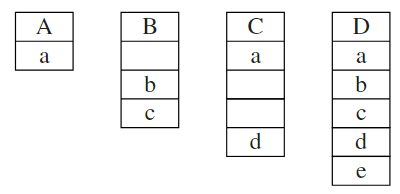
\includegraphics[width=0.309\textwidth]{pic/CP14/Multiple inheritance of data fields}
    \caption{Multiple inheritance of data fields.}
    \label{fig:Multiple inheritance of data fields}
\end{figure}

优化: 可以看出存在许多空的 slot 被浪费了. 我们可以把 fields 在内存上合并, 转而在每个类的 class descriptors 中记录各个 field 的真实偏移量. 如 \textbf{Figure} \ref{fig:Field offsets in descriptors} 所示. 

\begin{figure}[!htb]
    \centering
    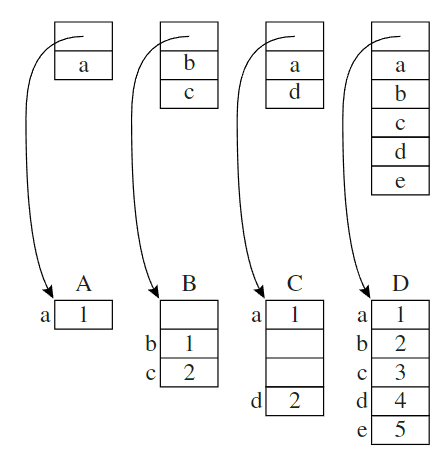
\includegraphics[width=0.22\textwidth]{pic/CP14/Field offsets in descriptors}
    \caption{Field offsets in descriptors}
    \label{fig:Field offsets in descriptors}
\end{figure}

由于类的数量远少于对象(类的实例)数量, 所以这样能节省空间. 不过这种优化导致每个 field 的具体偏移不固定了, 因此需要在运行时在 class descriptor 中动态查找(lookup) field 的真实偏移量.

\subsubsection{Method dispatch}
仍然使用图染色. 直接把 method 名混合进上述的图中, 一起染色; 也就是不仅记录 field 的偏移量, 也记录 method 的地址. 也有动态查找的开销. 

不过, 并非所有时候都可以静态知晓所有类的存在并统筹规划. 

解决方案: Hashing. 其实就是又包了一层新表, 允许通过 field/method 的名字本身索引到 field offset 或 method address. 更简单地说, 原先是 \mintinline{c++}{OffsetOrAddr[]} , 现在是 \mintinline{c++}{hashmap<Name, OffsetOrAddr>} .

\begin{itemize}
    \item Ftab(field table): field offset 或 method address (之前就有的)
    \item Ktab(key-table): 记录注册过的名字(因为有哈希冲突的问题, 需要确认名字是否真的匹配)
\end{itemize}

若要在 object $c$ 获取 field $b$, 编译器会:
\begin{enumerate}
    \item 在 $c$ 的 0 偏移处(开头)找到 class descriptor $d$.
    \item 从偏移量 $d+Ktab+hash_b$ 获取函数名 $f$
    \item 对比 $f$ 是否与 $b$ 相同
    \item 从偏移量 $d+Ftab+hash_b$ 获取 field $b$
    \item 获取 field $b$ 的内容. 
\end{enumerate}

\begin{figure}[!htb]
    \centering
    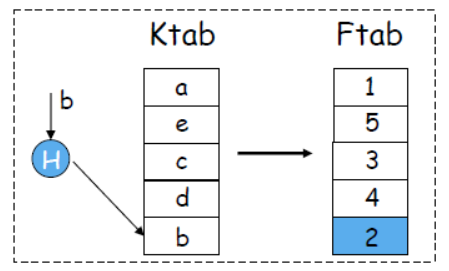
\includegraphics[width=0.309\textwidth]{pic/CP14/class descriptor}
    \caption{class descriptor}
\end{figure}


\subsection{Testing Class Membership}
每个类都是一种类型. 派生类可以看作一种 sub-type. 在进行类型转换时: 
\begin{itemize}
    \item upcast: 派生类转为基类. 永远是安全的.  在这种转换中相当于“丢失”了一些信息, upcast 后能调用/访问的 method/field 变少了. 
    \item downcast: 反之, 基类转为派生类不一定安全. 冒然转换就可能通过错误的 offset 访问到错误的、越界的内存, 很危险. 
\end{itemize}

Membership test: 为了安全的类型转换, 需要测试某个对象是否是某个类的实例. 

如何判断 $x$ 是不是类 $C$ 的实例?

朴素(慢)的做法: 递归地检查 $x$ 的 class descriptor (记作 $x.0$) 开始的继承链 $x.0$, $x.0.super$, $x.0.super.super$, $x.0.super.super.super$, $\dots$ 如果发现某个是 $C$ 的 class descriptor 则 $x$ 是 $C$ 的实例; 否则如果到最上层($\dots super==NIL$)仍未发现, 则说明不是 $C$ 的实例. 

更快的做法: display. 每个 class descriptor 储存一个 display, 也就是一个足够长(比最长继承链长)的定长列表, 记录对象的整条继承链. 就像: 
\begin{minted}{text}
    0: Object
    1: GrandparentClass
    2: ParentClass
    3: MeClass
    4: (nil)
    5: (nil)
    ...
\end{minted}
我们可以给每个类一个专属的数字 ID (例如对于 SI, 可以按照继承关系树的 BFS 序为每个类编号), 然后 display 中储存这些 ID 代表类. 由于对每个类, 其继承关系的嵌套深度在编译期已知, 因此可以立刻找到需要比较 display 中的哪一项. 例如, 假设 MeClass 的继承深度是第 3 层, 要检查 $x$ 是否为MeClass的实例, 只需检查 $x$ 的继承深度是否大于等于 3, 且 $x.0.display[3]$ 是否指向 MeClass 的 class descriptor 即可. 


\subsection{Private Fields and Methods}
private field/method: 私有的 field/method 只能被类的其他 method 访问/调用, 而不能被外部调用. 这是封装思想的体现: 调用者不该知道内部实现细节. 
通过类型检查确保私密性(privacy): 每个访问/调用处检查是否 private.
